\documentclass[lmodern, utf8, diplomski, numeric]{fer}
\usepackage{booktabs}

\begin{document}

\thesisnumber{1115}

\title{DUBOKE KONVOLUCIJSKE NEURONSKE MREŽE ZA RASPOZNAVANJE ZNAKOVA}

\author{Matija Ilijaš}

\maketitle

% Ispis stranice s napomenom o umetanju izvornika rada. Uklonite naredbu \izvornik ako želite izbaciti tu stranicu.
\izvornik

% Dodavanje zahvale ili prazne stranice. Ako ne želite dodati zahvalu, naredbu ostavite radi prazne stranice.
\zahvala{}

\tableofcontents

\chapter{Uvod}
Uvod rada. Nakon uvoda dolaze poglavlja u kojima se obrađuje tema.

\chapter{Optičko prepoznavanje znakova}

\chapter{Umjetne neuronske mreže}

Umjetna neuronska mreža je algoritam strojnog učenja inspiriran strukturom i funkcionalnošću ljudskog mozga. Zasniva se na paralelnoj obradi podataka, te vrlo dobro rješava sve probleme kod kojih postoji složena nelinearna veza ulaza i izlaza. Radi s velikim brojem parametara i varijabli, te može raditi s nejasnim podacima što ju čini robusnom na pogreške. Zbog svoje robusnosti, najčešća primjena neuronske mreže je u raspoznavanju uzoraka, obradi slike i govora, nelinearnom upravljanju itd.

Mreža se sastoji od tri vrste sloja: ulaznog, izlaznog, te skrivenog koji povezuje prethodna dva. Čvorišta, tzv. neuroni, skrivenog sloja povezani su težinskim vezama s ulaznim i izlaznim neuronima. Dvije su faze rada umjetnih neuronskih mreža: učenje (treniranje) i obrada podataka (eksploatacija). Učenje je iterativan postupak predočavanja ulaznih primjera i očekivanog izlaza pri čemu dolazi do postupnog prilagođavanja težina veza neurona. Nakon što se težine skrivenog sloja prilagode postupkom treniranja, eksploatacijom neuronske mreže može se za do tad neviđeni ulazni primjer dobiti pripadajući izlaz.


\chapter{Duboko učenje}

Duboko učenje se u zadnjih nekoliko godina pojavilo kao novo obečavajuće područje statističkog strojnog učenja. Iako je sama ideja prezentirana u radovima Yann Lecuna i George Hintona 1980ih godina, duboko učenje je postalo predmetom istraživanja tek relativno nedavno. Razlog tome je bio tad nedovoljno jak hardware za učenje velikih modela karakterističnih za taj pristup. Koncept dubokog učenja zasniva se na učenju korisnih prezentacija podataka povezanih u obliku hijerarhije. Ideja je djelomično inspirirana vizualnim korteksom mozga sisavaca koji se sastoji od niza procesirajućih elemenata koji obrađuju vizualni podražaj. Dokaz da duboko učenje u nekoj mjeri oponaša vizualni korteks su i nedavna istraživanja gdje su se naučene značajke pokazale slične onima u korteksu. Glavna karakteristika algoritama dubokog učenja je velik broj slojeva kroz koje ulazni podatak mora proći do izlaza, gdje se prvi dio prolaza može zamisliti kao formiranje hijerarhijskog prikaza podatka, a drugi kao proces klasifikacije. Time jedan algoritam dubokog učenja ustvari preuzima zadatak izvlačenja korisnih značajki iz podataka te zadatak klasifikacije. Kod učenja algoritma cijeli se taj postupak uči na temelju podataka, te se time gubi potreba za ručnim definiranjem značajki podataka. 

\section{Hijerarhijski prikaz podataka}

Slika se može klasifikatoru prikazati na mnogo načina, od kojih je najjednostavniji vektor vrijednosti intenziteta piksela. Apstraktniji prikaz bio bi recimo skup rubova na slici, a još apstraktniji skup različitih oblika. Neki prikazi olakšavaju klasifikatoru proces učenja, a različiti problemi klasifikacije zahtijevaju razvijanje različitih prikaza odnosno značajki ulaznih podataka. Stoga  se tradicionalno razvijanje rješenja problema klasifikacije sastoji od dva dijela, razvijanja kvalitetnih značajki koje olakšavaju učenje te razvijanja klasifikatora. 

Proces razvoja kvalitetnih značajki podrazumijeva promatranje svojstva ulaznih podataka te naglašavanje onih koja su maksimalno diskriminantna. Napredak u točnosti klasifikacije većim dijelom se ostvarivao razvijanjem boljih značajki, tako je na primjer značajni napredak u prepoznavanju čovjeka ostvaren razvijanjem HoG značajki koje su dobro opisivale lokalne oblike te u isto vrijeme bile invarijantne na  promjene osvijetljenja i geometrijske transformacije. No s obizrom da se takav postupak razvijanja značajki bazira na ljudskom promatranju podataka, dolazi do gubitka informacija koje čovjek nije u stanju vidjeti. 

Kako bi se koristile sve informacije iz podataka, potrebne su metode koje određuju diskriminantne značajke izravno iz skupa podataka. Među popularnijim metodama tog tipa su metoda linearne diskriminantne analize (LDA) te metoda glavnih komponenata (PCA). Linearna diskriminantna analiza pronalazi prikaz podataka koji maksimalno diskriminira podatke različitih klasa, dok metoda glavnih komponenata prikazuje podatke kao linearnu kombinaciju linearno nekoreliranih varijabli koje imaju najveću varijancu.

Istraživanja vizualnog korteksa mozga sisavaca pokazala su da vizualni podražaj prolazi kroz više procesirajućih slojeva koji tvore hijerarhiju gdje svaki dodatni sloj predstavlja dodatnu razinu apstrakcije.  Značajke dobivene prethodno navedenim metodama predstavljaju jednu razinu apstrakcije, te se mogu zamisliti kao imitacija najnižeg sloja vizualnog korteksa. Ideja dubokog učenja inspirirana je vizualnim korteksom te se zasniva na učenju korisnih prezentacija podataka povezanih u obliku hijerarhije razina apstrakcije. Cilj dubokog učenja je razviti što kvalitetniji hijerarhijski prikaz objekata klasifikacije uz pomoć velike količine podataka.

\section{Učenje dubokih mreža}

Kao što je ranije spomenuto ideja dubokog učenja je naučiti hijerarhiju značajki iz podataka. S obzirom da to zahtijeva nekoliko dodatnih slojeva mreže, kompleksnost dubokih modela značajno je veća od standarnih. Poznato je da količina potrebnih podataka za kvalitetno učenje modela raste proporcionalno sa brojem njegovih slobodnih parametara. Stoga je za učenje dubokih mreža potrebno za red veličine više podataka nego kod učenja standarnih klasifikatora. Nedovoljna količina podataka za učenje, te nedovoljno jak hardware za učenje tako velikih modela, razlog su zašto duboko učenje nije zaživjelo 1980-ih godina kada je prvi put predstavljeno kao ideja. Dolazak specijaliziranih razvojnih alata za brzo učenje mreža na grafičkim karticama, kao i sve veća količina dostupnih podataka za učenje, omogućili su da duboko učenje u zadnjih nekoliko godina pokaže svoj potencijal na raznim problemima strojnog učenja.
Jedna od velikih prednosti dubokog učenja je što uz metode nadziranog učenja ima razvijene i metode nenadziranog učenja. 
  
\subsection{Nenadzirano učenje}

Sve veća količina podataka postaje dostupna za učenje, no velikim dijelom radi se o neoznačenim podatcima. Kako bi se i ti podatci iskoristili potrebne su metode nenadziranog učenja.
Kao što je ranije spomenuto, duboki modeli predstavljaju hijerarhiju značajki podataka u prvih nekoliko slojeva, a jednu razinu apstrakcije moguće je postići metodom glavnih komponenata (PCA). Stoga se u teoriji postavlja pitanje da li uzastopnim primjenjivanjem PCA metode možemo dobiti traženu hijerarhiju. Odgovor na to pitanje je da ne možemo, a razlog tome je linearnost metode glavnih komponenata. Uzastopnom linearnom transformacijom konačno se uvijek dobiva linearna transformacija.





\subsection{Nadzirano učenje}





\chapter{Duboke konvolucijske neuronske mreže}

\chapter{Implementacija}

U sklopu ovog rada razvijen je sustav za učenje i testiranje različitih arhitektura neuronskih mreža. Prilikom razvijanja takvog sustava bilo je važno zadovoljiti dva glavna uvjeta: brzo učenje novih arhitektura na velikoj količini podataka te detaljna analiza rada naučenih mreža. Iz tog razloga sustav je podijeljen na dva podsustava razvijena sa zasebnim alatima. Podsustav zadužen za učenje implementiran je u razvojnom alatu Torch koji omogućuje paralelno izvođenje procesa učenja na grafičkoj kartici. Podsustav koji provodi analizu rada naučenih mreža implementiran je u jeziku C++ korištenjem OpenCV biblioteke.

\section{Sustav za učenje}

Kako bi cijeli proces istraživanja različitih arhitektura mreža i podataka bio što efikasniji, potrebno je prije svega imati brzi sustav za učenje. Učenje velikih arhitektura na velikoj količini podataka može trajati tjednima, pa i mjesecima, sekvencijalnim računanjem na standarnom procesoru računala. Stoga je tek pojavom kvalitetnih biblioteka, koje omogućuju optimizirano paralelno računanje na grafičkoj kartici, postalo moguće provoditi istraživanje u području dubokog učenja. 
Osim brzine učenja, važna je i jednostavnost definiranja parametara mreže koja se uči, kao i parametara samog procesa učenja. Kod implementacije ovog rada odabran je razvojni alat Torch zbog svoje jednostavnosti i brzine, ali i podrške velikih kompanija kao što su Facebook i Google, koje nerijetko dijele korisne implementacije sa zajednicom. 

\subsection{Torch razvojni alat}

Prilikom odabira razvojnog alata uzeti su u obzir i alati Caffe i Theano. Možda najpopularniji alat za duboko učenje Caffe ima izrazito jednostavno sučelje za odabir parametara mreže i procesa učenja, no kao posljedica toga teško je raditi promjene u postojećoj implementaciji u svrhu istraživanja ili razvoja. Theano s druge strane pruža puno manju razinu apstrakcije te ostavlja mogućnost lake izmjene većine implementacije, no postaje nepraktičan kod česte upotrebe standarnih algoritama.
Torch je po razini apstrakcije negdje između prethodno navedenih alata, dovoljno je niske apstrakcije za laku izmjenu implementacije kod razvoja i istraživanja, ali ima i sučelje za standarne algoritme koje ga čini praktičnim. 

Brzina samog izvođenja procesa učenja na grafičkim karticama velikim dijelom ovisi o pozadinskoj implementaciji paralelnog računanja koja je za sve navedene alate otprilike podjednako brza, te se toliko često mijenja da nema smisla uspoređivati njihove brzine. S druge strane, važan faktor kod odabira alata je podrška akademske zajednice i industrije s obzirom da o tome ovisi koliko brzo se razvijaju implementacije novih koncepata. Torch ima implementaciju za većinu novih koncepata u dubokom učenju zbog podrške kompanija kao što su Google, Facebook i Twitter.  Tako je primjerice implementirana relativno nova metoda Dropout za regularizaciju prilikom učenja mreže te ReLU funkcija prijelaza koja je pokazale bolje rezultate od standardne sigmoidalne funkcije u nedavnim istraživanjima.

Sama implementacija Torcha podijeljena je na dva dijela. Sve računske operacije na grafičkoj kartici napisane su kao C/CUDA implementacija za maksimalnu brzinu, dok je ostatak funkcionalnosti implementiran u skriptnom jeziku LuaJIT za lakše korištenje alata.  

\subsection{Definiranje arhitekture}
	
Neuronska mreža je u Torch alatu definirana kao model koji se sastoji od sekvencijalno povezanih slojeva koji vrše različite računske operacije.
Tako bi na primjer standarna neuronska mreža s jednim skrivenim slojem bila definirana kao sekvencijalni niz prikazan na Slici ???. 

\begin{figure}[ht!]
\centering
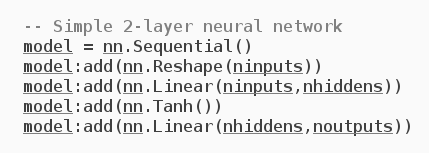
\includegraphics[width=9cm]{slike/nn_model.png}
\caption{}
\end{figure}

Primjer duboke konvolucijske mreže definirane kao Torch model prikazan je na Slici ???.

\begin{figure}[ht!]
\centering
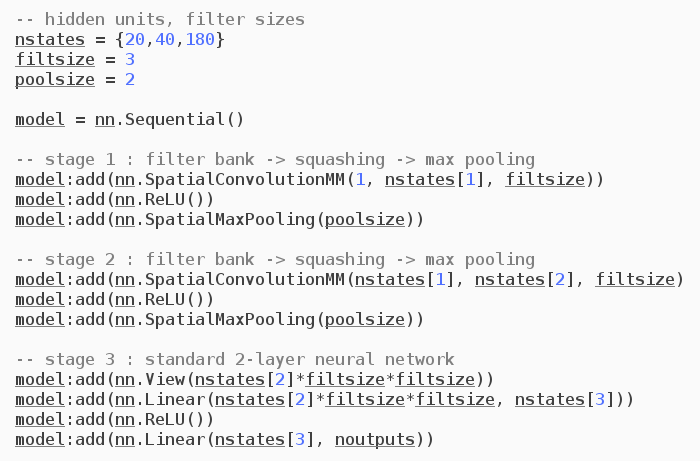
\includegraphics[width=16cm]{slike/cnn_model.png}
\caption{}
\end{figure}

\subsection{Definiranje parametara učenja}




\section{Sustav za testiranje}



\chapter{Rezultati}

\chapter{Zaključak}
Zaključak.

\bibliography{literatura}
\bibliographystyle{fer}

\begin{sazetak}


\kljucnerijeci{Ključne riječi, odvojene zarezima.}
\end{sazetak}

\engtitle{Deep convolutional neural networks for character recognition}
\begin{abstract}
Abstract.

\keywords{Keywords.}
\end{abstract}

\end{document}
